%% This LaTeX-file was created by Marco Kienzle (Marco.Kienzle@gmail.com)
%% 
%% Do not edit this file unless you know what you are doing.

% This latex template was created to produce document that will be transformed into MS Word document.
% The command to do so is 
% latex article.tex
% bibtex article
% latex2rtf -Z3 -P /usr/local/share/latex2rtf/cfg/:/tmp/latex2rtf-1.9.16a/scripts/ article.tex

\documentclass{article}
%\documentclass{nrc2}
%\journal{cjfas}

\usepackage[dvips]{color}

%\usepackage{bbding}
\usepackage[round]{natbib}
\usepackage{setspace}
\usepackage{amsmath}
\usepackage{graphicx}
%\usepackage{psfig}
\usepackage{verbatim}
\usepackage{rotating}
\usepackage{multirow}
\usepackage{longtable}
\usepackage{booktabs}
\usepackage{subfigure}
\usepackage{lineno}
\usepackage{url}
\renewcommand{\baselinestretch}{1.5} % set space between lines to 1.5

\setlength{\oddsidemargin}{0.5cm}
\setlength{\evensidemargin}{0.5cm}
\setlength{\textwidth}{17cm}
%\setlength{\textheight}{23cm}
%\addtolength{\oddsidemargin}{-3cm}
%\addtolength{\evensidemargin}{-3cm}

\usepackage{fancyhdr}
\pagestyle{fancyplain} %Note the \fancyplain command !!!
%\renewcommand{\chaptermark}[1]{\markboth{#1}{}}
%\renewcommand{\sectionmark}[1]{\markright{#1}{}}
\lhead[\fancyplain{E}{EE}] {\fancyplain{}{}}
\chead[\fancyhead{}{}]{\fancyplain{}{—Draft—}}
\cfoot [ ] {\copyright \hspace{0.1cm} The State of Queensland (through the Department of Agriculture and Fisheries) [2015] \begin{center} \thepage \end{center}}

\begin{document}

\linenumbers

\title{Hazard function models to estimate mortality rates affecting fish populations by maximum likelihood using age data,\\ with application to the sea mullet ({\it Mugil cephalus}) fishery on the Queensland coast (Australia)}

%\author{Marco Kienzle\footnote{Queensland Dept of Agriculture, Fisheries and Forestry, Ecosciences Precinct, Joe Baker St, Dutton Park, Brisbane, QLD 4102, Australia; \newline University of Queensland, School of Agriculture and Food Sciences, St. Lucia, QLD 4072, Australia}, Jason McGilvray\footnote{Queensland Dept of Agriculture, Fisheries and Forestry, Ecosciences Precinct, Joe Baker St, Dutton Park, Brisbane, QLD 4102, Australia} and You-Gan Wang\footnote{University of Queensland, Centre for Applications in Natural Resource Mathematics, School of Mathematics and Physics, St. Lucia, QLD 4072, Australia}}
\author{Marco Kienzle\footnote{Queensland Dept of Agriculture, Fisheries and Forestry, Ecosciences Precinct, Joe Baker St, Dutton Park, Brisbane, QLD 4102, Australia; \newline University of Queensland, School of Agriculture and Food Sciences, St. Lucia, QLD 4072, Australia}}

\maketitle

\abstract{Fisheries management agencies around the world collect age data for the purpose of assessing the status of natural resources in their juridiction. Estimates of mortality rates are central to assess the sustainability of fish stocks exploitation. Survival analysis has seldom been applied to fisheries research despite its widespread use in medical research and engineering to estimate failure rates. In this paper, we present a variety of hazard functions to model the dynamic of a fishery and estimate by maximum likelihood all parameters necessary for a stock assessment (including natural and fishing mortality rates as well as gear selectivity) from a sample of fish age. These methods were tested by Monte Carlo simulations to assert that they provide un-biased estimates of these quantities. An application to the Queensland's sea mullet fishery (Australia) dataset provided an estimate of natural mortality equal to 0.319 $\pm$ 0.165 year$^{-1}$.


%% Survival analysis has seldomed be used in this area of research despite estimate fish mortality ratesSurvival analysis was applied to fisheries catch at age data to develop maximum likelihood estimators for stock assessment. This new method estimated natural mortality, fishing mortality and catchability from typical catch at age matrices. Monte Carlo simulations suggested estimates were unbiased and provided a better fit than the traditional multinomial approach. 

%% Application to a dataset from Queensland's sea mullet fishery (Australia) estimated natural mortality to be equal to 0.319 $\pm$ 0.165 year$^{-1}$.
}

\section{Introduction} One of the purposes of stock assessment is to estimate mortalities affecting fish stocks. This task is much easier for species that can be aged compared to, for example crustaceans, which aging is not possible. The reason lies in that mortality and longevity are inversely related hence age is a measure, albeit inverse, of mortality. The central mortality model used in fisheries research was proposed by Baranov to describe the variation of the number of fish belonging to a cohort through time \citep{quin99b}. This deterministic exponential model has a statistical counterpart in the form of the exponential probability distribution function which first and second moments quantify the relationship between longevity (age) and mortality rate \citep{cow98b}. Adopting a statistical view of this problem allowed to develop maximum likelihood estimators \citep{Burnb03} of parameters of importance to stock assessment scientists. The branch of statistics focused on survival analysis has created and refined methods to estimate mortality rates \citep{cox84b} which are widely applied in the fields of medical research and engineering. \\ 

%The present article describes an application of survival analysis to fisheries catch at age data.
Despite the commonalities between survival analysis for medical and fisheries research, this theory has seldom been applied to animal ecology \citep{Pollock1989}: to our knowledge, there hasn't been any application to fish age data for the purpose of stock assessment. In this manuscript, we described how to apply survival analysis to create likelihood functions of catch at age for the purpose of estimating natural and fishing mortalities as well as gear selectivity. We started with a simplistic example of constant natural and fishing mortality to introduce fundamental concepts from survival analysis before moving to more sophisticated cases leading to its application to real data from the sea mullet fishery in Queensland (Australia). The proposed methods were tested with simulated data to characterize some of their properties and their capacity to estimate population dynamic parameters of interest. Finally, the application to the mullet fishery case study provided specific estimates of natural mortality, catchability and selectivity. \\


\section{Materials and methods} 

Fish aging is possible thanks to a little bone called the otolith which is present in their ears. An otolith accumulate materials and increases in size throughout the entire lifespan of a fish. Microscopic analyses of sections of an otolith shows a series of marks, similar to tree rings, that can be used to assign each individual to a specific age-group.\\

Most fisheries institute around the world have a sampling program dedicated to collect a representative sample of fish each year to determine the distribution of age of any species of interest. In most cases, the data are binned into age-groups of width 1 year. For this reason, we split the lifespan of cohorts from their birth ($t \in [0;\infty]$) into $n$ yearly intervals from $a_{1}=0$ to the maximum age of $a_{n+1}$ years. While the theory presented in this document used that particular subdivision of time ($t$), un-equal ones also applies. In fact, an un-equal subdivision of time was used for the sea mullet case study.
 


\subsection{The likelihood for constant natural and fishing mortality rates} 
           \input{ConstantNaturalAndFishingMortality.tex}

\subsection{Estimating catchability and natural mortality}
           \input{EstimatingQandM.tex}

\subsection{Estimates from catch at age matrix using fishing mortality separability}
           This section describes an application of survival analysis to matrices of catch at age, developed for the purpose of estimating catchability ($q$), selectivity at age ($s(t)$) and constant natural mortality ($M$). The matrix ($S_{i,j}$) containing a sample of fishes aged to belong to a particular age-group $j$ in year $i$ contains $n+p-1$ cohorts. These cohorts were indexed by convention using $k$ ($k \in [1, n+p-1]$) and an increasing number $r_{k}$ ($ 1 \leq r_{k} \leq {\rm min}(n,p)$) identifying incrementally each age-group (see Appendix p.~\pageref{Appendix:DefinitionsOfMathematicalSymbols} for more information). Each matrix $S_{i,j}$ has two cohorts with only 1 age-group representing them.\\

The derivation for a single cohort were the same as those presented in the previous section, here reproduced with indexations relative to a single cohort and accounting for selectivity

\begin{equation}
g_{k}(t; \theta) = \frac{q \ s(t) \ E(t) \times e^{-Mt-q\int_{0}^{t} s(t) \ E(t) \ dt}}{\sum_{l=1}^{r_{k}} \frac{q \ s_{k,l} \ E_{k,l}}{M+q \ s_{k,l} \ E_{k,l}} \bigl ( e^{-M \ a_{k,l}-q\int_{0}^{a_{k,l}}s(t) \ E(t) \ dt} - e^{-M \ a_{k,l}-q\int_{0}^{a_{k,l+1}}s(t) \ E(t) \ dt} \bigr )} 
\end{equation}
\newline
The likelihood function of a catch at age matrix was built using each pdf specific to each cohort ($g_{k}(t; \theta)$):

\begin{equation}
\mathcal{L} = \prod_{k=1}^{n+p-1} \prod_{l=1}^{r_{k}}  \bigl ( \int_{t=a_{k,l}}^{t=a_{k,l+1}} g_{k}(t; \theta) \ dt \bigr ) ^ {S_{k,l}}
\end{equation}

The expression above is equivalent to 
\begin{equation}
\mathcal{L} = \prod_{i,j} P_{i,j} ^ {S_{i,j}}
\end{equation}

\noindent where the $P_{i,j}$ are the probabilities of observing a fish of a given age $j$ in year $i$ given by the hazard model. In this likelihood, the $P_{i,j}$ sum to 1 along the cohort instead of summing to 1 for each year as described for the multinomial likelihood in \cite{Four82a}. \\

This method was implemented in R \citep{R} in the package Survival Analysis for Fisheries Research (SAFR). Numerical applications of this method are available from \url{https://github.com/mkienzle/SurvivalAnalysisForFisheries}. %using the following commands: {\bf library(SAFR); example(llfunc3); example(llfunc4); example(llfunc5);}.\\


\subsection{Monte Carlo simulations}
           Methods to estimate mortality and selectivity from a matrix containing a sample of number at age were tested with simulated datasets to characterize their performance. Variable number of cohorts ($n+p-1 = 25$, 35 or 45); maximum age ($p=8$, 12 or 16 years) and sample size of age measurement in each year varying from 125 to 2000 increasing successively by a factor 2. The simulated datasets were created by generating an age-structure population using random recruitment for each cohort, random constant natural mortality, random catchability and random fishing effort in each year (Tab.~\ref{tab:SimulationParameters.tex}). A catch at age matrix was calculated using a logistic gear selectivity with 2 parameters: 

\begin{equation}
s_{a_{i}} = \frac{1}{1  + {\rm exp}( \alpha - \beta \times a_{i})}
\end{equation}

Several sampling strategies were implemented to assess how it affected mortality estimates. To test estimators derived from survival analysis, one would like to draw randomly from the probability distribution. This is obviously impossible in the real world because field biologists never have in front of them a entire cohort to chose from. Nevertheless, we implemented a sampling strategy (sampling strategy 1) that randomly selected from the entire simulated catch at age dataset as a benchmark. In the real world, samples can be drawn by accessing only a single year-class of every cohort every year, so the second strategy implemented was to simulate a random selection of a fixed number of sample ($N$) each year (sampling strategy 2). Finally, the third strategy investigated was to apply a weighting by the estimated total catch at age ($\hat{C}_{i,j}$) to the sample of number at age in the sample ($S_{i,j}$) -- sampling strategy with weighting :

\begin{equation}
\hat{C}_{i,j} = p_{i,j} \odot C_{i} \otimes v(j)
\end{equation}

\noindent where $p_{i,j}$ is the proportion at age (see Appendix p.~\pageref{Appendix:DefinitionsOfMathematicalSymbols}), $C_{i}$ is a column vector containing the total number of fish caught in each year $i$ and $v(j)$ is a row vector of 1's. A weighted sample ($S^{*}_{i,j}$) was obtained using the fraction of total catch sampled
\begin{equation}
S^{*}_{i,j} = \hat{C}_{i,j} \times \frac{\sum_{i,j} S_{i,j}}{\sum_{i} C_{i}}
\end{equation}

Note that $\sum_{i,j} S_{i,j} = \sum_{i,j} S^{*}_{i,j}$.\\
%implemented a strategy that collected a number of samples in proportion to fishing effort (SS3).\\

%A sample of $N$ individuals per year was drawn at random from this matrix of catch at age, creating a matrix of sampled number at age data, with dimensions $n \times p$ containing $n \times N$ data, that were processed with survival analysis methods described in previous sections.\\ %Multiplicative white noise of magnitude 0\%, $\pm$ 10\%, ..., $\pm$ 50\% was applied to these simulated data to assess how it influenced uncertainty on parameter estimates.

Comparisons with the multinomial likelihood proposed by \cite{Four82a} were made using differences in negative log-likelihood between that method and the survival analysis approach described in the present article. Simulated catch were used to calculate the proportion of individual at age, constraining them to sum to 1 in each year. This method to calculate proportions for the multinomial likelihood was regarded as the best case scenario because we expect any estimation algorithm based on the multinomial likelihood to, at best, match exactly the simulated catch at age. The logarithm of these proportions were then multiplied by the simulated age sample (weighted or not depending on the case) to calculate the log-likelihood as described in \cite{Four82a}. This quantity was compared to that calculated using the survival analysis approach to determine which model best fitted the simulated data. This comparison ignored the number of parameters used in each model as the Akaike criteria would. The multinomial likelihood requires $n+p-1$ more parameters to be estimated than the survival analysis because the former requires an estimate of recruitment for each cohort in order to calculate the proportion at age in the catch.


\subsection{A case study: Queensland's sea mullet fishery}
           The straddling Sea Mullet ({\it Mugil cephalus}) population stretches along the east coast of Australia, with most landings occurring between 19$^{o}$S (approx. Townsville) and 37$^{o}$S (roughly the border between New South Wales and Victoria). Following recommendations from \cite{Bell2005r}, an existing (1999--2004) scientific survey design was modified from 2007 onward to include both estuaries and ocean habitats in order to provide representative demographic statistics for Queensland component of this fishery. The number of fish at age obtained by otolithometry (Tab.~\ref{tab:Mullet-NbAtAge}) were analyzed to estimate natural mortality, catchability and gear selectivity. \\

Sea Mullet are thought to spawn in oceanic waters adjacent to ocean beaches from May to August each year. By convention, the birth date was assumed to be on July 1$^{st}$ each year. Opaque zones are thought to be deposited on the otolith margin during spring through early summer (September to December). Biologists have come to the conclusion that the first identifiable opaque zone is formed 14 to 18 months after birth, and all subsequent opaque zones are then formed at a yearly schedule \citep{Smith2003}. Each fish in the sample was assigned an age-group based on opaque zone counts and the amount of translucent material at the margin of otolith. Age-group 0--1 comprised fish up to 18 months old ($a_{1}=18$ months) while all subsequent age-groups spanned 12 months ($a_{2} = 30$ months, $a_{3}= 42$ months, etc ...).\\

Sensitivity of survival analysis estimates to these data, a matrix containing 7 years and 16 age-groups, were performed by truncating the dataset in 2 ways to assess the robustness of the method to varying number of years and age-groups. The first truncation removed the last and last-two years of data to evaluate the sensitivity of parameters estimates to addition/omission of data in order to anticipate possible effects of future addition of newly available data. The second truncation removed older age-groups from 10--11 to 15--16 to evaluate the importance of few old fish on natural mortality estimates as one could think {\it a priori} that these longer-lived individuals provided a lot of information on mortality.\\




\section{Results}

    \subsection{Method tests using simulated data}
               Natural mortality estimates were biased using a fixed number of sample per years while they were not when numbers at age in the samples were weighted by total catch (Fig~\ref{fig:Estimating-NaturalMortality}). This correction to the sample data reduced considerably the uncertainty on natural mortality and remove almost completely bias: a small of amount of bias was still noticeable at the extremity of the range of natural mortality (0.1--1.0) tested. Increasing number of samples reduced uncertainty associated with natural mortality estimates. \\ 

Estimates of catchability were much more consistent across the range of value (1--10 10$^{-4}$) tested between methods (Fig.~\ref{fig:Estimating-Catchability}). The bias of the un-weighted approach was often similar to that of the weighted one. But uncertainty associated with the former approach were much larger than the latter. They appeared to be fairly in-sensitive to sample size. \\



    \subsection{Mortality estimates for sea mullet}
               Applying survival analysis to age data from a sample of Sea Mullet weighted by total yearly catch, catchability was estimated to be equal to 7.055 $\pm$ 2.724 $10^{-5}$ per boat-day (Tab.~\ref{tab:Sensitivity-CatchabilityToMulletDataTruncation}). Natural mortality for Sea Mullet was estimated to 0.319 $\pm$ 0.165 year$^{-1}$ using the entire dataset (comprising 2013 and 16 age-groups, Tab.~\ref{tab:Sensitivity-NaturalMortalityToMulletDataTruncation}). The sensitivity analysis showed consistent estimates with the removal of 1 or 2 years and up to 6 age-groups: catchability estimates varied between [7.054; 7.126] 10$^{-5}$ with mean equal to 7.079 $10^{-5}$ boat.days$^{-1}$ and natural mortality estimates varied between [0.319; 0.382] with mean equal to 0.336 year$^{-1}$. This sensitivity analysis suggested that the presence of age-groups in the dataset with fewer, sparse observations increased the uncertainty of both catchability and natural mortality estimates.\\

The maximum likelihood matrix of probabilities ($P_{i,j}$) associated with the weighted observations at age in the sample ($S^{*}_{i,j}$) were presented in Tab.~\ref{tab:MaximumLikelihoodProbabilitiesOfMulletAgeSampleWeightedByTotalCatch}. They illustrate that the construction of the likelihood estimator using this survival analysis relied on probabilities summing to 1 along the cohort instead of summing to one along rows and across cohorts, as previously proposed to develop the multinomial likelihood of age data by \cite{Four82a}. Note that 2 cohorts in the dataset were described by a single observation (top-right and bottom-left corner of the matrix in Tab.~\ref{tab:MaximumLikelihoodProbabilitiesOfMulletAgeSampleWeightedByTotalCatch}) which did not provide any information to estimate mortality rates, as represented by their associated probability equal to 1.\\

Maximum likelihood estimates of gear selectivity, catchability and natural mortality were slightly affected by weighting the sample of observed number at age by total yearly catch (Tab.~\ref{tab:EffectOfWeightingOnMulletEstimates}), suggesting that variation of catch within $\pm$ 12\% of the coefficient of variation influenced on the outcome of the analysis (Tab.~\ref{tab:Mullet-NbAtAge}).



\section{Discussion} This application of survival analysis to fisheries catch at age data provides a novel likelihood approach to estimate natural, fishing mortalities and gear selectivity. Testing this method with simulated data showed that it provided un-biased estimates of natural mortality and catchability over a wide range of simulated values. This likelihood method should find its place naturally in integrated stock assessment \citep{Maunder201361} as it provide an efficient way of dealing with catch at age data.\\

% There are advantage of reducing the number of age-groups when number of individual become small because there is a lot of uncertainty where there are little data which increased uncertainty on other parameters

%%%%%%%%%%%%%%%%%%%%%%%%%%%%%%%%%%%%%%%%%%%%%%%%%%%%%%%%%%%%%%%%%%%%%%%%%%%%%%%%%%%%%%%%%%%%%%%%%%%%%%%%%%%%%%%%%%%%%%%%%%%%%%%%%%%%%%%%%%%
%%% Simulations
%%%%%%%%%%%%%%%%%%%%%%%%%%%%%%%%%%%%%%%%%%%%%%%%%%%%%%%%%%%%%%%%%%%%%%%%%%%%%%%%%%%%%%%%%%%%%%%%%%%%%%%%%%%%%%%%%%%%%%%%%%%%%%%%%%%%%%%%%%%
The simulations used a logistic gear-selectivity to generate and fit the data although we would have preferred to generate data from one of the many possible gear-selectivity functions or even using non-parametric procedures. Simulations showed that gear selectivity was most difficult to estimate. The sea mullet case study was in fact not fitted with a logistic curve but selectivity was estimated through a tedious process to search each proportion retained at age that best fitted the data as measured by the likelihood. This tedious process could not be automatised into the simulation-testing framework to provide automatic identification of gear-selectivity. Therefore it was left out for a future work. Criticisms that this somewhat simplified the problem would be correct. But the current article was designed as an introduction to these methods in fisheries research not one that solves all problems at once. The purpose of writing the present manuscript was to provide likelihood methods allowing to identify the correct gear-selectivity. \\ %, as shown by the sea mullet case study, by comparing many possibilities and assessing which minimize the likelihood. The current simulations provided an evaluation of the properties of these estimators assuming the shape of gear-selectivity was known. 



%%%%%%%%%%%%%%%%%%%%%%%%%%%%%%%%%%%%%%%%%%%%%%%%%%%%%%%%%%%%%%%%%%%%%%%%%%%%%%%%%%%%%%%%%%%%%%%%%%%%%%%%%%%%%%%%%%%%%%%%%%%%%%%%%%%%%%%%%%%
%%% Sea mullet
%%%%%%%%%%%%%%%%%%%%%%%%%%%%%%%%%%%%%%%%%%%%%%%%%%%%%%%%%%%%%%%%%%%%%%%%%%%%%%%%%%%%%%%%%%%%%%%%%%%%%%%%%%%%%%%%%%%%%%%%%%%%%%%%%%%%%%%%%%%

% about sea mullet stock structure
Parasite data suggested that the bulk of sea mullet caught in Queensland fishery is based on local fish populations and not migrating from NSW \citep{Lester2009129}. While genetic analyses could not identify differences in single nucleotide polymorphism between samples from south QLD and NSW \citep{kruck2013a}.\\

% estimate of natural mortality
The sensitivity analysis to data truncation showed a weak trend in increasing uncertainty associated with natural mortality as more older age-groups containing few observations were added to the analysis suggesting that lack of information with those create large uncertainties on gear selectivity estimates which translate into greater estimates of natural mortality uncertainty.\\

%%%%%%%
% Future work
%%%%%%%
This survival analysis approach to fisheries catch at age data can be further expanded to provide an estimator of recruitment.


\section*{Acknowledgements} I would like to thank the staff in the Long Term Monitoring Program of Queensland Department of Agriculture and Fisheries for their hard work collecting otoliths and measuring age. In particular, I am in debt to Jason McGilvray for introducing and explaining the intricacies of the mullet dataset to me. I am grateful to W.N. Venables from the Commonwealth Scientific and Industrial Research Organisation and N. White from Queensland University of Technology for the many discussions on the topic of applying survival analysis to fisheries data. 


\clearpage
\newpage
%% %% Bibliography
\bibliography{a-JLong,Biblio}
%\bibliographystyle{plain}
\bibliographystyle{plainnat}
%\bibliographystyle{ieeetr}
%\bibliographystyle{apalike}

\clearpage
\newpage
\section*{Figures}

%% Testing how the method can estimate natural mortality
 \begin{figure}[!ht]
     \includegraphics[scale=0.6, angle = -90]{../Results/Graphics/Estimating-NaturalMortality.ps}
      \caption{Comparison between simulated natural mortality (x-axis) and estimated (y-axis) using a random sample of the matrix of catch (strategy 1); a random sample from each year separately (strategy 2) and the same sample weighted by yearly total catch (strategy 2 - weighted samples). Each panel correspond to an increasing number of samples per year varying from 125 to 2000.}
     \label{fig:Estimating-NaturalMortality}
   \end{figure}

%% Testing how the method can estimate catchability
 \begin{figure}[!ht]
     \includegraphics[scale=0.6, angle = -90]{../Results/Graphics/Estimating-Catchability.ps}
      \caption{Comparison between simulated catchability (x-axis) and estimated (y-axis) using a random sample of the matrix of catch (strategy 1); a random sample from each year separately (strategy 2) and the same sample weighted by yearly total catch (strategy 2 - weighted samples). Each panel correspond to an increasing number of samples per year varying from 125 to 2000.}
     \label{fig:Estimating-Catchability}
   \end{figure}

%% Compare negative log-likelihood from survival analysis to multinomial from Fournier and Archibald (1982)
 \begin{figure}[!ht]
     \includegraphics[scale=0.6, angle = -90]{../Results/Graphics/ComparisonOfNegLL.ps}
      \caption{Difference between the negative log-likelihood ($-{\rm log}(\mathcal{L})$) from survival analysis (SA) and multinomial (ML) as a function of the number of sample per year. Each panel represents a particular sampling strategy.}
     \label{fig:ComparisonOfNegLL}
   \end{figure}

\clearpage
\newpage
\section*{Tables}
% by marco 11/10/2014

\begin{table}[ht]
\centering
\begin{tabular}{lll}
  \hline
Variable type & Distribution & Parameters \\
  \hline
recruitment               & uniform & min=1e6, max=1e7   \\
natural mortality         & uniform & min=0.1, max=0.8 \\
catchability              & uniform & min=3e-4, max=1e-3 \\
fishing effort            & uniform & min=1e3, max=5e3   \\
gear selectivity $\alpha$ & uniform & min=8, max=12      \\
gear selectivity $\beta$  & uniform & min=1, max=3       \\
   \hline
\end{tabular}
\caption{Distribution and range of value taken by different type of random variable in simulations.}
\label{tab:SimulationParameters.tex}
\end{table}

\input{Tables/Mullet-NbAtAgeEDITED.tex}

\input{"/home/mkienzle/mystuff/Work/DEEDI/Biometry services/Fisheries/Mullet/Results/Tables/MulletModelComparisonEDITED.tex"}
%% latex table generated in R 3.1.1 by xtable 1.7-1 package
% Thu Dec 11 07:41:01 2014
\begin{sidewaystable}[ht]
\centering
\begin{tabular}{rlllllll}
  \hline
 & 10 & 11 & 12 & 13 & 14 & 15 & 16 \\ 
  \hline
2012 & 7.093 $\pm$ 3.254 & 7.101 $\pm$ 0.973 & 7.126 $\pm$ 1.029 & 7.095 $\pm$ 3.195 & 7.116 $\pm$ 1.636 & 7.095 $\pm$ 7.221 & 7.095 $\pm$ 6.491 \\ 
  2013 & 7.054 $\pm$ 1.176 & 7.055 $\pm$ 1.237 & 7.056 $\pm$ 1.367 & 7.056 $\pm$ 1.384 & 7.056 $\pm$ 2.393 & 7.056 $\pm$ 2.131 & 7.055 $\pm$ 2.724 \\ 
   \hline
\end{tabular}
\caption{Sensitivity of catchability estimates (x$10^{-5}$ boat-day$^{-1}$) to data truncations. Rows indicate the most recent year of data and columns the maximum age-group included in the analysis.} 
\label{tab:Sensitivity-CatchabilityToMulletDataTruncation}
\end{sidewaystable}

%% latex table generated in R 3.1.1 by xtable 1.7-1 package
% Thu Dec 11 07:41:01 2014
\begin{sidewaystable}[ht]
\centering
\begin{tabular}{rlllllll}
  \hline
 & 10 & 11 & 12 & 13 & 14 & 15 & 16 \\ 
  \hline
2012 & 0.334 $\pm$ 0.117 & 0.36 $\pm$ 0.052 & 0.382 $\pm$ 0.05 & 0.339 $\pm$ 0.066 & 0.382 $\pm$ 0.046 & 0.337 $\pm$ 0.248 & 0.337 $\pm$ 0.239 \\ 
  2013 & 0.319 $\pm$ 0.075 & 0.319 $\pm$ 0.083 & 0.32 $\pm$ 0.091 & 0.32 $\pm$ 0.091 & 0.32 $\pm$ 0.154 & 0.319 $\pm$ 0.132 & 0.319 $\pm$ 0.165 \\ 
   \hline
\end{tabular}
\caption{Sensitivity of natural mortality estimates (in year$^{-1}$) to data truncations. Rows indicate the most recent year of data and columns the maximum age-group included in the analysis.} 
\label{tab:Sensitivity-NaturalMortalityToMulletDataTruncation}
\end{sidewaystable}


%% latex table generated in R 3.1.1 by xtable 1.7-1 package
% Tue Dec  9 09:13:19 2014
\begin{table}[ht]
\centering
\begin{tabular}{lcc}
  \hline
 & un-weighted & weighted \\ 
  \hline
q & 6.153 $\pm$ 1.504 & 7.055 $\pm$ 2.724 \\ 
  M & 0.396 $\pm$ 0.038 & 0.319 $\pm$ 0.165 \\ 
  $s_{1}$ & 0.002 $\pm$ 0 & 0.002 $\pm$ 0 \\ 
  $s_{2}$ & 0.074 $\pm$ 0.008 & 0.085 $\pm$ 0.015 \\ 
  $s_{3}$ & 0.399 $\pm$ 0.02 & 0.419 $\pm$ 0.04 \\ 
  $s_{4}$ & 0.909 $\pm$ 0.047 & 0.882 $\pm$ 0.074 \\ 
  $s_{5}$ & 1 $\pm$ 0.033 & 1 $\pm$ 0.078 \\ 
  $s_{6}$ & 1 $\pm$ 0.053 & 1 $\pm$ 0.076 \\ 
  $s_{7}$ & 0.96 $\pm$ 0.091 & 0.981 $\pm$ 0.098 \\ 
  $s_{8}$ & 0.96 $\pm$ 0.116 & 0.981 $\pm$ 0.115 \\ 
  $s_{9}$ & 0.961 $\pm$ 0.131 & 0.982 $\pm$ 0.104 \\ 
  $s_{10}$ & 0.961 $\pm$ 0.154 & 0.982 $\pm$ 0.162 \\ 
  $s_{11}$ & 0.961 $\pm$ 0.157 & 0.982 $\pm$ 0.798 \\ 
  $s_{12}$ & 0.962 $\pm$ 0.322 & 0.982 $\pm$ 0.878 \\ 
  $s_{13}$ & 0.962 $\pm$ 0.532 & 0.982 $\pm$ 1.925 \\ 
  $s_{14}$ & 1 $\pm$ 0.505 & 1 $\pm$ 0.741 \\ 
  $s_{15}$ & 1 $\pm$ 1.06 & 1 $\pm$ 1.555 \\ 
  $s_{16}$ & 1 $\pm$ 1.039 & 1 $\pm$ 1.199 \\ 
   \hline
\end{tabular}
\caption{Comparison of maximum likelihood parameters estimates for the mullet fishery using un-weighted or weighted samples of age data.} 
\label{tab:EffectOfWeightingOnMulletEstimates}
\end{table}

\input{"/home/mkienzle/mystuff/Work/DEEDI/Biometry services/Fisheries/Mullet/Results/Tables/BestParameterEstimatesEDITED.tex"}
% latex table generated in R 3.1.1 by xtable 1.7-1 package
% Tue Dec  9 09:13:19 2014
\begin{sidewaystable}[ht]
\centering
\begin{tabular}{rrrrrrrrrrrrrrrrr}
  \hline
 & 1 & 2 & 3 & 4 & 5 & 6 & 7 & 8 & 9 & 10 & 11 & 12 & 13 & 14 & 15 & 16 \\ 
  \hline
1 & 0.0025 & 0.0968 & 0.3290 & 0.5339 & 0.5739 & 0.5750 & 0.5691 & 0.5690 & 0.5690 & 0.5689 & 0.5712 & 0.5766 & 0.5874 & 0.6192 & 0.6886 & 1.0000 \\ 
  2 & 0.0028 & 0.1071 & 0.3233 & 0.3812 & 0.2833 & 0.2595 & 0.2563 & 0.2599 & 0.2599 & 0.2598 & 0.2598 & 0.2609 & 0.2633 & 0.2721 & 0.2800 & 0.3114 \\ 
  3 & 0.0025 & 0.0932 & 0.2835 & 0.3003 & 0.1615 & 0.1020 & 0.0920 & 0.0932 & 0.0945 & 0.0945 & 0.0945 & 0.0945 & 0.0948 & 0.0972 & 0.0980 & 0.1008 \\ 
  4 & 0.0029 & 0.0938 & 0.2811 & 0.3072 & 0.1525 & 0.0702 & 0.0437 & 0.0403 & 0.0408 & 0.0414 & 0.0414 & 0.0414 & 0.0414 & 0.0422 & 0.0422 & 0.0426 \\ 
  5 & 0.0057 & 0.1212 & 0.3167 & 0.3412 & 0.1759 & 0.0749 & 0.0339 & 0.0216 & 0.0200 & 0.0202 & 0.0205 & 0.0205 & 0.0205 & 0.0208 & 0.0207 & 0.0207 \\ 
  6 & 0.0258 & 0.2458 & 0.4212 & 0.3912 & 0.1973 & 0.0871 & 0.0365 & 0.0169 & 0.0108 & 0.0100 & 0.0101 & 0.0102 & 0.0102 & 0.0104 & 0.0103 & 0.0103 \\ 
  7 & 1.0000 & 0.9742 & 0.7486 & 0.4547 & 0.1957 & 0.0843 & 0.0367 & 0.0157 & 0.0073 & 0.0047 & 0.0043 & 0.0044 & 0.0044 & 0.0045 & 0.0044 & 0.0044 \\ 
   \hline
\end{tabular}
\caption{Maximum likelihood probabilities ($P_{i,j}$) of the observed mullet sample age dataset weighted by total catch.} 
\label{tab:MaximumLikelihoodProbabilitiesOfMulletAgeSampleWeightedByTotalCatch}
\end{sidewaystable}


\clearpage
\newpage
\appendix
\section{Appendix}

\subsection{Definitions of some mathematical symbols}
\input{DefinitionsOfMathematicalSymbols.tex}

%\clearpage
%\newpage
%\section*{Programs code}

\end{document}









